\documentclass[12pt, a4paper]{article}
\usepackage[utf8]{inputenc}
\usepackage[T1]{fontenc}
\usepackage{fullpage}
\usepackage{hyperref}
\usepackage[parfill]{parskip}
\usepackage{natbib}
\usepackage{url}
\usepackage{amsmath}
\usepackage{graphicx}
\graphicspath{{images/}}
\usepackage{vmargin}
\usepackage[nottoc,numbib]{tocbibind}


\title{The Delivery Man}	% Title
\author{André Le Blanc, Joel Wallin}
\date{\today}			

\makeatletter
\let\thetitle\@title
\let\theauthor\@author
\let\thedate\@date
\makeatother

%----------------------------------
% Wizard stuff
%----------------------------------
\begin{document}

\begin{titlepage}
	\centering
    \vspace*{0.5 cm}
    %\includegraphics[width=5cm,height=5cm,keepaspectratio]{deadrop_text.png}\\[0.5 cm]
    %\includegraphics[width=5cm,height=5cm,keepaspectratio]{deadrop_logo.png}\\[1 cm]
    %\textsc{\huge Artificial Intelligence (1DL340) fall 2016}\\[2.0 cm]
	%\textsc{\Large \today}\\[0.5 cm]
	\rule{\linewidth}{0.2 mm} \\[0.4 cm]
	{ \huge \bfseries \thetitle}\\  
	\rule{\linewidth}{0.2 mm} \\[1.5 cm]
    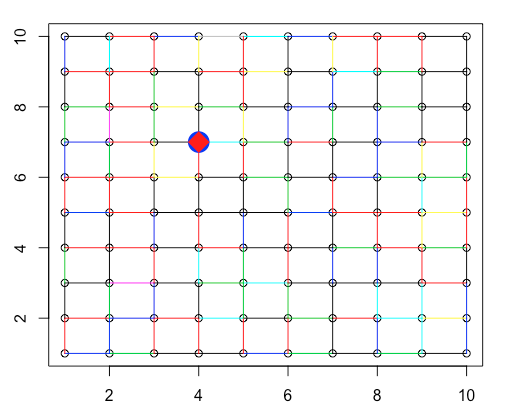
\includegraphics[width=10cm,height=5cm,keepaspectratio]{images/ADONE.png}\\[0.5 cm]
    
    \textsc{\Large Lab Group 14:}\\[0.5 cm]
	\begin{minipage}{0.4\textwidth}  
    \begin{align*}
	&\text{André Le Blanc}    &&\text{910930-3850}\\
	&\text{Joel Wallin}  &&\text{941123-3134}\\
	\end{align*}
	\end{minipage}\\[2 cm]
\end{titlepage}


\newpage
\tableofcontents
\newpage

\section{Introduction}

For this lab assignment the task was to guide a delivery man through a grid to his packages and to their destination. The deliveryman has to traverse a 9x9 square grid with nodes in every corner, and the edges between the nodes (roads) have a cost for traversing them, ranging from 0 to 5. During the simulation traffic conditions for the roads can change every time the delivery man makes a move. An A* algorithm is used to determine the next move of the deliveryman, and it will have to adapt to the changing conditions in order to find an optimal route.

Once the simulation is over the program returns the number of steps it took for the delivery man to complete his tasks. By running multiple simulations with different variations of the A* algorithm and varying strategies, an optimized setup has been found that minimizes the number of steps the delivery
man has to take.


\subsection{Tools and methods}

The programming language used for this assignment was R together with RStudio as the development environment. R is a high level multiparadigm language designed for statistical computing\cite{rLang}. Git and GitHub was used for version control and sharing files. 


\section{Algorithms}

Finding and optimizing a path for the deliveryman to the destination is done with the help of the A* algorithm. However other methods are used before A* can be applied, such as algorithms that determine which package should be picked up next.

\subsection{A theoretical overview of A*}

A* is a pathfinding algorithm developed from Dijkstra’s algorithm in 1968 by Nils Nilsson, Bertram Raphael and Peter Hart\cite{nils}. It promises to find the shortest path between two nodes in a well defined system given that such a path exists. A* is a best first search algorithm meaning that it explores a graph or a weighted graph by expanding the most promising node until it finds its destination\cite{amit}\cite{aStar}.

At the heart of the A* algorithm we have the following function :
\begin{equation} \label{eq:1}
f(n) = g(n) + h(n)
\end{equation}
In equation \ref{eq:1} $n$ represents the last node on a path. $g(n)$ is the cost of getting to that node from the starting node. $h(n)$ is a heuristic for the distance between node $n$ and the destination. A* tries to minimize the $f(n)$ function and chooses to expand on the nodes where $f(n)$ has the lowest value. $g(n)$ is generally obtained by adding together the costs of getting to each node on the shortest path between the starting point and node n\cite{amit}\cite{aStar}.

Finding a good implementation of $h(n)$ is a science in itself. If the heuristic between node $n$ and the destination always is zero then:
\begin{equation} \label{eq:2}
f(n) = g(n)
\end{equation}
If a scenario like in equation \ref{eq:2} occurs, it means that A* will be an implementation of Dijkstra’s algorithm since A* is Dijkstra’s algorithm with a heuristic that helps A* choose the most efficient node to expand. A* will still find the shortest path but the algorithm will be more costly to run\cite{amit}.

If $h(n)$ has a higher value, but the value is still lower than the cost of going from node $n$ to the destination the algorithm will be more efficient expanding fewer nodes that are unnecessary to expand. In an ideal world $h(n)$ is equal to the cost of traveling from node $n$ to the destination. In this case A* will only expand nodes that are on the path between $n$ and the destination. In the unfortunate case where $h(n)$ is greater than the cost of getting from node $n$ to the destination it is possible that the A* algorithm finds a path that is less efficient than the optimal path between $n$ and the destination\cite{amit}. Therefore it is extremely important that the relationship in equation \ref{eq:3} holds.
\begin{equation} \label{eq:3}
h(n) \leq g(n)
\end{equation}

\subsection{Implementation of A*}

Graph search was chosen to represent the problem space, which includes a visited set (closed nodes). A frontier is also used, containing all nodes that can be reached from an already expanded node, excluding nodes that are closed. The frontier is implemented as a sorted list in relation to the lowest cost calculated by the function $f(n)$ in equation \ref{eq:1} (where $n$ is a node), so the node with the lowest $f(n)$ value will be at the head of the list.

Nodes are added starting from the right of the current node, then left, followed by up and lastly down. If there is a tie between two nodes, which happens if two nodes have the same $f(n)$ value, the first node to be expanded will be the first node in the frontier. Choosing the next node to expand is then simple, just extract the head of the frontier and then repeat the process until the goal is reached.

%This is an arbitrary approach but since it does not affect the accuracy of the algorithm we didn't implement a more complex tie breaking algorithm. Sometimes zigzagging tie breaking algorithms are preferred for aesthetic reasons but these cost in terms of extra calculation and don't provide a shorter path. 

In order to calculate $f(n)$ as in equation \ref{eq:1}, both $g(n)$ (the cost) and $h(n)$ (the heuristic) has to be defined. Two different heuristics were experimented with, the Manhattan distance \cite{manD} and the Euclidean distance \cite{eucD}. The cost had two configurations as well, the first approach was to define the cost of a node as the cost of its parent added by its individual edge cost. Which is defined in equation \ref{eq:4}, where the cost of the parent is denoted as $g(p)$ and the edge cost from the parent to the current node is denoted as $c$.
\begin{equation} \label{eq:4}
g(n) = g(p) + c
\end{equation}
The second approach was to minimize the impact of the edge costs by only giving a node the cost of its individual edge plus the number of steps required to get to the node (the path). Which is defined in equation \ref{eq:5}, where the number of steps from the start to the current node is denoted as $s$.
\begin{equation} \label{eq:5}
g(n) = s + c
\end{equation}
%The Manhattan distance function was developed for calculating the distance traveled in Manhattan, an entirely grid based area. On Manhattan you can only travel along the x axis or the y axis. The Manhattan distance is the absolute value of the difference between the current location on the x axis minus the location of the destination on the x axis plus the absolute value of the difference between the current location on the y axis minus the location of the destination on the y axis.

%Euclidean distance is the the distance as the crow flies. We calculated this distance using the Pythagorean theorem. 

%On a grid Manhattan distance is a more accurate heuristic than Euclidean distance. 

\subsection{Non A* Strategies}

The program could just perform A* once and take that path to its destination. The chosen strategy is to instead perform A* every time the delivery man has taken one step on the grid. The program therefore calculates the optimal path for every iteration between the start and the destination.

One of the things that the program does not use A* for is choosing what package to pick up next. The package which has the smallest Manhattan distance from the current node is chosen and A* is then performed to find a path.

Waiting with a chance $p$ ranging from $1.0$ to $0.05$ when the cost of a road is high was experimented with. Including waiting if the A* algorithm determined that a detour is the best option.

%performed A* after every move.

%We have implemented two algorithms for finding the nearest package, one using Manhattan distance and one using Euclidean distance. The algorithm that uses the Manhattan distance algorithm chooses the package that has the lowest Manhattan distance between the current location and the package.



\section{Results}

In order to measure the effectiveness of different heuristics, A* strategies and non A* strategies, hundreds of different runs were executed with different variations of these parameters. Then the different strategies were evaluated by looking at the expected value (the mean in this case) and the standard deviation of their series of results.

Using Manhattan distance or Euclidean distance as the heuristic did not yield any noticeable improvements. However there was a difference between a function that uses the Euclidean distance instead of the Manhattan distance for choosing which package to go to. The Euclidean distance is shorter than the actual distance that is needed to be traveled if the route to the package is diagonal. This means that the Euclidean algorithm will underestimate the distance to packages that are diagonally placed in relation the the current location. The Euclidean algorithm is hence less efficient in this case than the Manhattan distance. 

Strategies that de-emphasized the cost in the A* algorithm as in equation \ref{eq:5}, did perform worse and penalizing high costs as in equation \ref{eq:4}, caused the delivery man to zigzag slightly more and to avoid costly paths. Which narrowly improved its performance. Figure \ref{mmp_mmd-box} is a comparison between these two approaches using a small sample size of 100 runs. Where penalizing the cost clearly performs better as its expected value is lower but with similar standard deviations.

\begin{figure}[!ht]
\centering
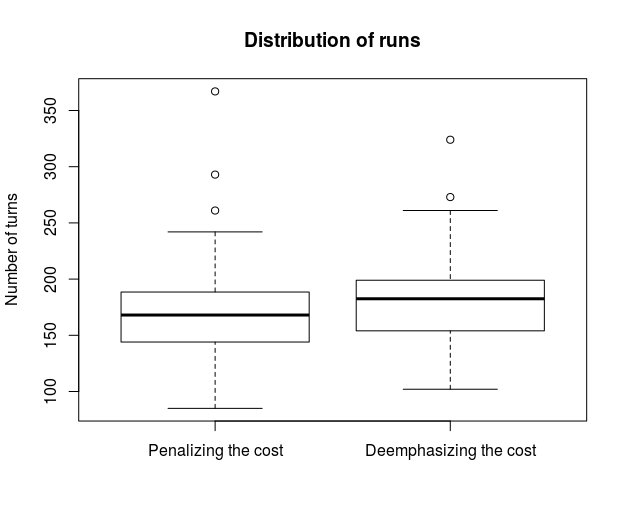
\includegraphics[width=10cm,height=10cm,keepaspectratio]{images/mmp_mmd-box.png}\\
\caption{Penalizing versus de-emphasizing high costs.}
\label{mmp_mmd-box}
\end{figure}
\vspace{2.5mm}

Waiting at a node when the cost is high did not improve the performance either. The car would stand still for too long, negating the benefits of waiting. Giving the car a probability $p$ of waiting if the cost was high still made it perform worse than not waiting, but made it preform better than waiting an extended period of time if the cost is high. In figure \ref{pp-box} it is clear by comparing with figure \ref{mmp_mmd-box} that waiting using this method is worse than not waiting. Both the expected value and the standard deviation is a lot higher.
%\newpage

\begin{figure}[!ht]
\centering
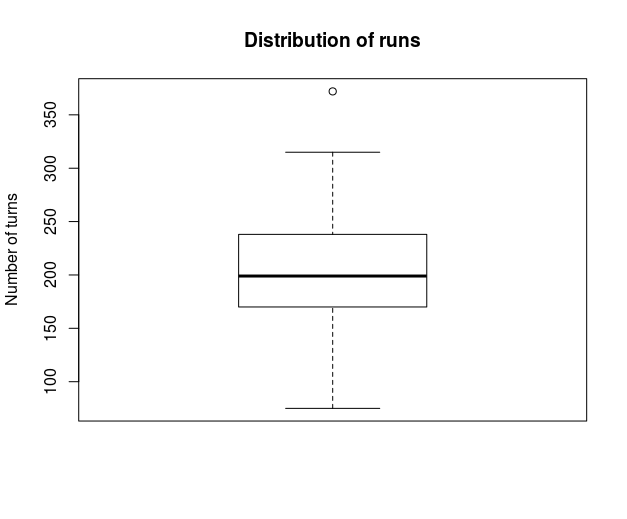
\includegraphics[width=10cm,height=10cm,keepaspectratio]{images/pp-box.png}\\
\caption{If the cost exceeds 4, wait with probability $p=0.2$.}
\label{pp-box}
\end{figure}
\vspace{2.5mm}

The final chosen setup was using the Manhattan distance as the heuristic and slightly penalizing high costs. 1,000 runs were executed and the results of those can be seen in figure \ref{mmp-box}. The expected value of the algorithm is: 170.53 steps and the standard deviation was: 40.865, giving a 95\% confidence interval of the expected value as $[167.997, 173.063]$.
%\newpage

%insert the histogram and box graph
%\begin{figure}[!ht]
%\centering
%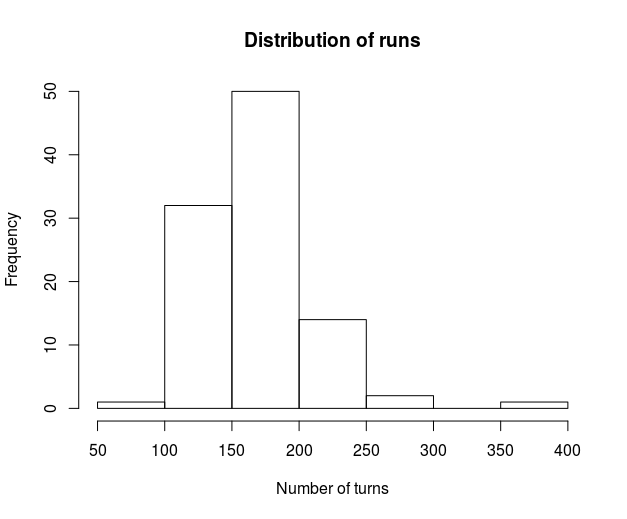
\includegraphics[width=10cm,height=10cm,keepaspectratio]{images/mmp-hist.png}\\
%\caption{Waiting 20\% of the time if the g cost of a road exceeds 4.}
%\label{mmp-hist}
%\end{figure}
%\vspace{2.5mm}

\begin{figure}[!ht]
\centering
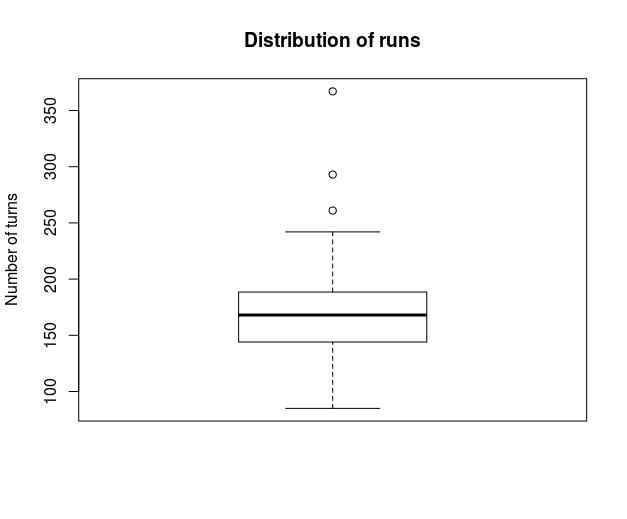
\includegraphics[width=10cm,height=10cm,keepaspectratio]{images/mmp-box.png}\\
\caption{Manhattan distance and penalizing cost.}
\label{mmp-box}
\end{figure}
\vspace{2.5mm}


\section{Discussion}
% why choose manhattan over euclidean, etc.
Using graph search for finding a path in the grid in this program is more natural due to the existence of loops in the graph. Even though the probability that the algorithm will consider a loop is fairly low. The reason Manhattan distance was chosen over the Euclidean distance or any other type of heuristic, was the fact that its value always is equal to the shortest distance to the destination. Making the heuristic ideal, as the A* algorithm will not have to expand too many unnecessary nodes, which gets more important if the search space increases. Finding an ideal heuristic was therefore quite simple, the difficult part was dealing with the ever-changing costs of the roads.

In this problem, the cost grows fast as the algorithm traverses the grid, while the heuristic decrease linearly. The cost is hence emphasized more when calculating the $f(n)$ value (as in equation \ref{eq:1}) of a node. This makes the car follow low costs to a greater extent. The car however still nearly always chooses a path with the lowest possible Manhattan distance due to detours seldom being worth it. This can be explained by looking at the provided code for the program. For every turn, the chance that the cost of a road will change is calculated through a uniform distribution of random numbers where the probability of the cost increasing is 10\% and the probability of the cost decreasing is 5\%. For every iteration the road conditions consequently will on average worsen. This also explains why waiting is almost never beneficial. Running the A* algorithm after every step of the delivery man also allows the program to adapt to the changing costs.

It is still possible to improve the performance of the traversing algorithm by doing more extensive analysis of the grid's state, ex. comparing paths between different packages with the Manhattan distance (or even A*) and choosing the order of packages which provides the shortest path. One such strategy that could be applied is to take nodes that keeps the delivery man in the same area as other nodes. Doing this minimizes the number of extra steps required, as there would be no unnecessary scenario where you waste steps by going back and forth in the grid because of a sub optimal route.

\section{Conclusion}

The best parameters for implementing an A* algorithm for this particular problem is to use the Manhattan distance as the heuristic and to slightly penalize high costs between nodes. And running the A* algorithm after every step the delivery man takes. Waiting is generally useless due to the costs of the roads tending to increase as time goes by. Which also favors A* going fairly straight towards the destination. Using graph search is also a better idea than tree search due to the existence of loops.

The implemented A* algorithm yields a better result than a person stepping through the graph unless the person extensively analyses the grid's state. This is due to the algorithm quickly and accurately finding a cost efficient path to its destination. That said, it is possible to improve the algorithm. As it is somewhat limited in its ability to determine an optimal order for picking up and delivering packages. So a person could still outperform the algorithm by doing time consuming analysis of the grid's state.


\raggedright
\bibliography{cit.bib}{}
\bibliographystyle{unsrt}

\end{document}
